%%%%%%%%%%%%%%%%%%%%%%%%%%%%%%%%%%%%%%%%%%%%
\section{PFS Coordinates and Calibrations in Commissioning Procedure}

\subsection{Definitions of Coordinates}
PFS has four coordinates used for fiber positioning: Sky Catalogue, Fixed Fiducial Fiber Coordinate (F3C), Cobra Coordinate, and Meteorology Camera System Coordinate (MCSC).

The definitions of each coordinates are as follows.

\paragraph{Sky Catalogue}
The sky targets such as galaxies and stars as well as sky backgrounds lie on this coordinates.
We describe the target positions using the equatorial coordinates $\bm{S}=(\alpha , \delta)$ in the unit of degree.
In the operation, we slew the telescope to a given field centered at $\bm{S}=(\alpha [ \degree ], \delta [ \degree ])$.
In this Field of View, the sky targets have a position on Sky Catalogue as the differential from the center: $\bm{S_k}=(\Delta \alpha _k [ \degree ], \Delta \delta _k [ \degree ])$.

\paragraph{Fixed Fiducial Fiber Coordinate (F3C)}
In order to calculate fiber positions at each exposures, 97 fixed fiducial fibers are used.
F3C is the coordinate from the viewpoint of these fibers.
In this coordinate, sky targets and fiber positions are described in the unit of mm: $\bm{X_k}=(x_k [ \mathrm{mm} ], y_k [ \mathrm{mm} ])$.
In practical, F3C is roughly defined as  mean plane of the top surface of the fixed fiducial fibers.
F3C resembles physical metrics of PFI (Prime Focal Instrument), but in fact it is {\it different} because the orientation between each fiducial fiber is constant in F3C.
For example, consider the case where the Focal Plane expands along with the increase of the temperature.
In such a case, the separation of the two fiducial fibers gets larger, whilst the separation in F3C doesn't change at all (see Figure \ref{fig:F3Cex1}).
% no distortion, no thermal expansion etc.

\begin{figure}[!ht]
\begin{center}
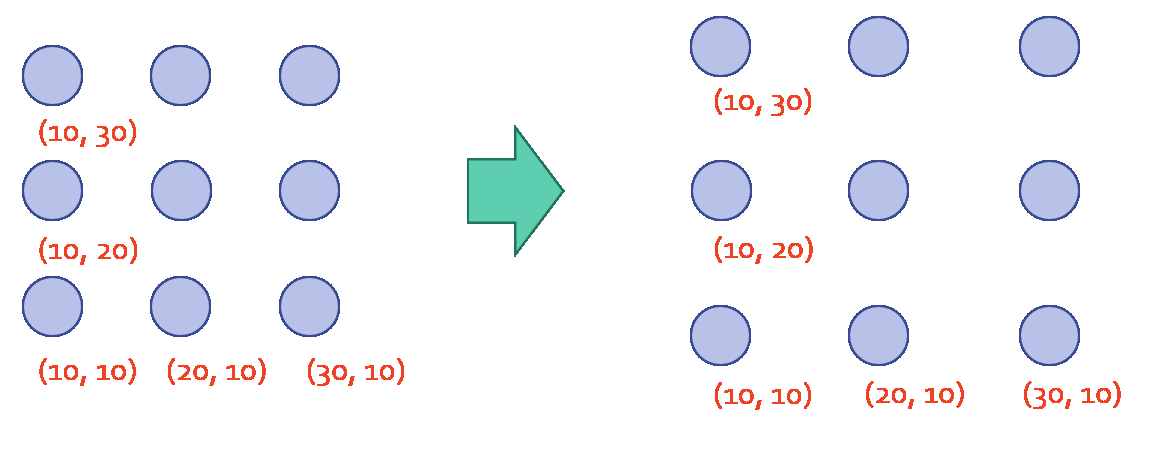
\includegraphics[width=100mm]{F3C_example1.eps}
\end{center}
\caption{An example of the change in physical metrics of fiducial fibers (blue circles).
The fiber positions in F3C are described in red letters.
}
\label{fig:F3Cex1}
\end{figure}

Another example explaining the difference between F3C and the physical metrics of PFI is the case where one of the fixed fiducial fibers happens to shift from the original position (Figure \ref{fig:F3Cex2}).
In such case, the positions of all fixed fiducial fibers are constant again.
Measure for this case is described in section \ref{sec:failures}.

\begin{figure}[!ht]
\begin{center}
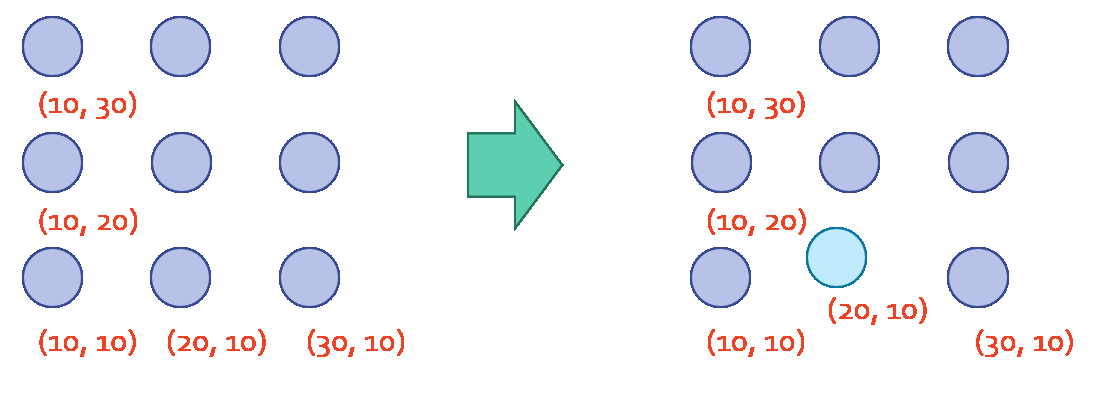
\includegraphics[width=100mm]{F3C_example2.eps}
\end{center}
\caption{Another example of the change in physical positions of fiducial fibers (blue and light-blue circles).
The fiber positions in F3C is described in red letters.
}
\label{fig:F3Cex2}
\end{figure}

\paragraph{Cobra Coordinates}
The fiber positioner ``cobra" is a two-axis motor; $\theta$ stage and $\phi$ stage.
The motion of each cobra is controlled by MPS (Movement Planning Software) with the two angles of these stage in degree.
We call the two angle as the Cobra Coordinates: $\bm{C_k}=(\theta _k [ \degree ], \phi _k [ \degree ])\;, [k=1,2,....,2394]$ .

\paragraph{Meteorology Camera System Coordinate (MCSC)}
The subsystem Meteorology Camera System calculates centroids of back-illuminated fibers.
Here, the centroids are determined as the position on CMOS sensor in the unit of pixels, equivalent to MCSC.
The centroids of the fibers, therefore, is determined in MCSC as $\bm{F_k}=(i_k [ \mathrm{pixel} ], j_k [ \mathrm{pixel} ])$.

\subsection{Observational Sequence and Definitions of Coordinate Transformations}\label{sec:ctsec}

\begin{figure}[!ht]
\begin{center}
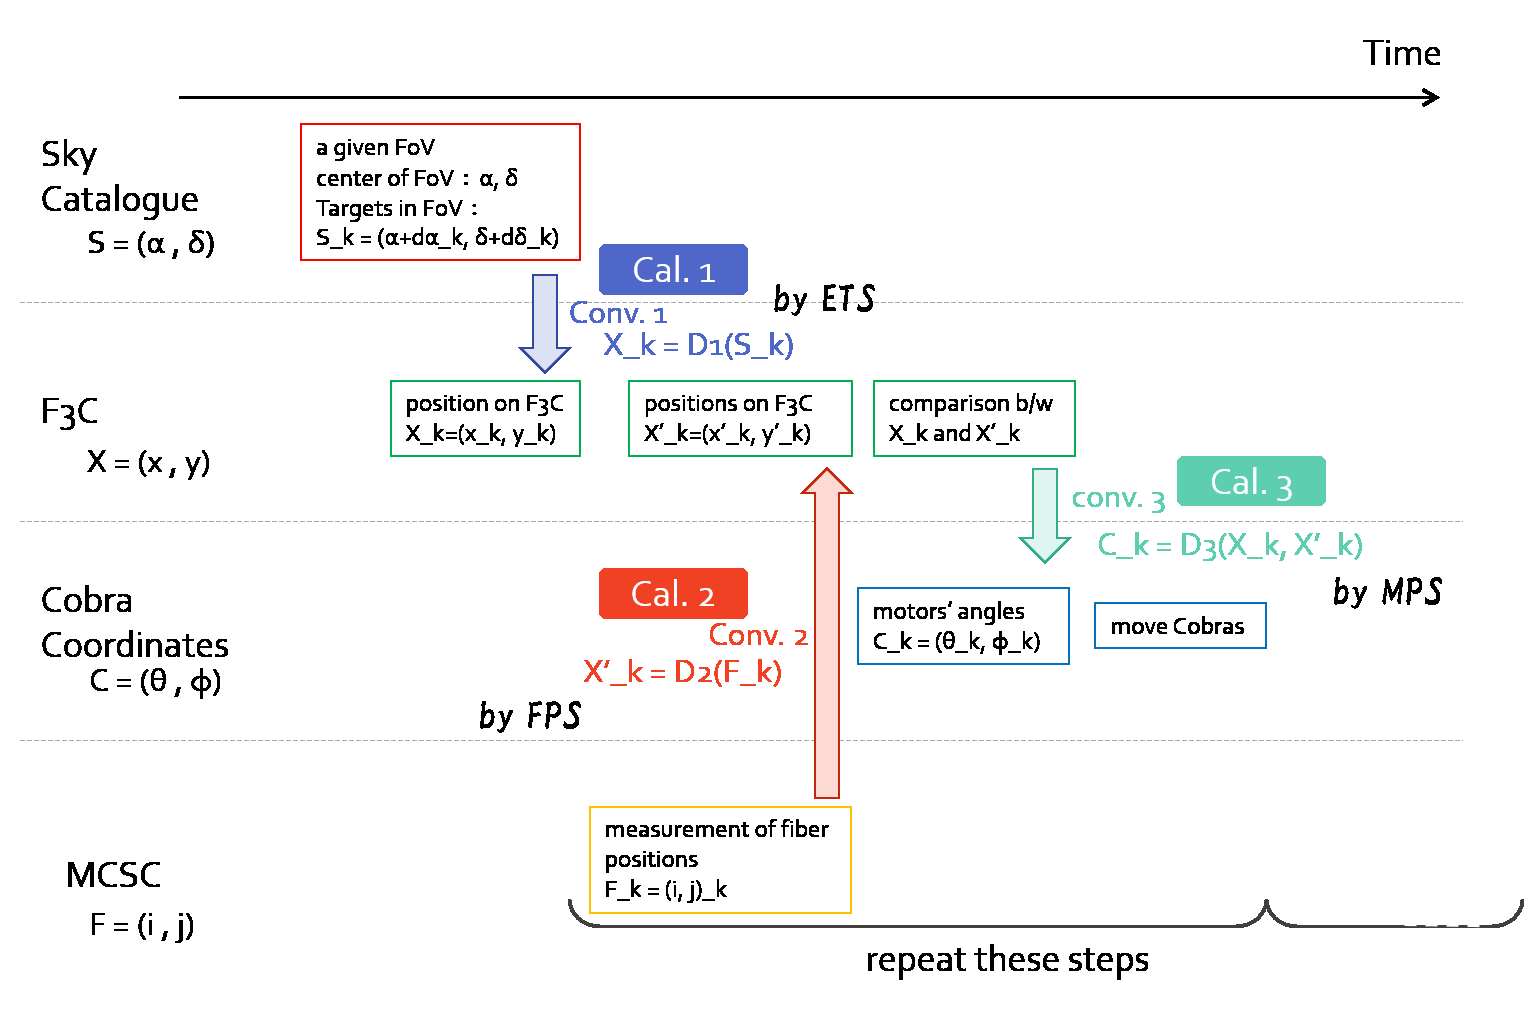
\includegraphics[width=150mm]{ObservationalSequence.eps}
\end{center}
\caption{PFS observational sequence and coordinates transformations.
}
\label{fig:obssec}
\end{figure}

Figure \ref{fig:obssec} shows observational sequence in particular during positioning fibers, and transformations of the above coordinates.
The procedure of fiber positioning is as follows:
\begin{enumerate}
%%% 1. sky
\item ETS (Exposure Time Sequencer) calculate the target positions $\bm{S_k}=(\Delta \alpha _k [ \degree ], \Delta \delta _k [ \degree ])$ in the observed field centered at $\bm{S}=(\alpha [ \degree ], \delta [ \degree ])$.
%%% 2. sky -> F3C
\item ETS transforms the target positions in Sky Catalogue to those in F3C using the telescope parameters at that moment ($Az, El, InR, T$).
We define this transformation as $D_1$.
That is,
\begin{equation}
\begin{array}{crcl}
& \bm{S_k}=(\alpha _k [ \degree ], \delta _k [ \degree ]) & \rightarrow & \bm{X_k}=(x_k [ \mathrm{mm} ], y_k [ \mathrm{mm} ]), \\
& & D_1 & \\
\mathrm{or} & \bm{X_k} &= & D_1(\bm{S_k}).
\end{array}
\end{equation}
In practical, firstly ETS calculates ($Az, El, InR$) at a given time for the filed centered at $\bm{S}$, or receives them from the telescope.
Then ETS calculates ($\Delta Az [ \degree ], \Delta El [ \degree ]$) of each target $\bm{S_k}$, as the offset of the field center.
This offset is transformed to the position on F3C using $D_1$.
That is,
\begin{equation}
\begin{array}{rcccl}
\bm{S_k}=(\alpha _k [ \degree ], \delta _k [ \degree ]) & \rightarrow & (\Delta Az [ \degree ], \Delta El [ \degree ]) & \rightarrow & \bm{X_k}=(x_k [ \mathrm{mm} ], y_k [ \mathrm{mm} ]), \\
& & & D_1 & \\
\end{array}
\end{equation}
%%% 3, MCSC -> F3C
\item\label{item:mcs2f3c} Take fiber image with MCS and measure fiber positions $\bm{F_k}=(i_k [ \mathrm{pixel} ], j_k [ \mathrm{pixel} ])$.
Then FPS (Fiber Positioning Sequencer) transforms the fiber positions in MCSC to those in F3C.
We define this transform as $D_2$.
That is,
\begin{equation}
\begin{array}{crcl}
& \bm{F_k}=(i_k [ \mathrm{pixel} ], j_k [ \mathrm{pixel} ]) & \rightarrow & \bm{X'_k}=(x'_k [ \mathrm{mm} ], y'_k [ \mathrm{mm} ]), \\
& & D_2 & \\
\mathrm{or} & \bm{X'_k} & = & D_2(\bm{F_k}).
\end{array}
\end{equation}
%%% 4. F3C -> MPS
\item\label{item:f3c2cobra} MPS calculates Cobra Coordinates to be commanded, by comparing the position of fibers $\bm{X'_k}$ and targets $\bm{X_k}$.
We call this transformation $D_3$.
\begin{equation}
\begin{array}{crcl}
& \bm{X_k}=(x_k [ \mathrm{mm} ], y_k [ \mathrm{mm} ]), \bm{X'_k}=(x'_k [ \mathrm{mm} ], y'_k [ \mathrm{mm} ]) & \rightarrow & \bm{C_k}=(\theta _k [ \degree ], \phi _k [ \degree ]) ,\\
& & D_3 & \\
\mathrm{or} & \bm{C_k} & = & D_3(\bm{X_k},\bm{X'_k}).
\end{array}
\end{equation}
%Comparing these positions, MPS derives the angles to move cobras $\bm{C_k}$:
%\begin{equation}
%\begin{array}{crcl}
% & \bm{C_k} & = & D_3(\bm{X'_k}) - D_3(\bm{X_k}).
%\end{array}
%\end{equation}
Then move Cobras following the derived angles $\bm{C_k}$.
%%% 5. repeat
\item Repeat \ref{item:mcs2f3c} and \ref{item:f3c2cobra} until the differential between the target and the fiber positions meets the required accuracy; $\Delta r_k= \sqrt{ \Delta x_k^2 + \Delta y_k^2} \leq 10 \;\mathrm{[um]}$ (TBC; {\tt REQ-SYS-553}).
FPS judges which fibers should be moved, and sends $\bm{X_k}$ and $\bm{X'_k}$ to MPS.
\end{enumerate} 

Formation of $D_1$ and $D_2$ is determined by the Project Office and stored to a designated repository (TBC), while $D_3$ is determined by JPL.
During the commissioning, the transformation functions $D_1$, $D_2$, and defined and/or calibrated, and calibration for $D_3$ are executed.
In the following section, these process are described.

%------------------------------
% subsection: calibrations
%------------------------------
\subsection{Calibrations of Coordinate Transformation during the Commissioning}\label{sec:coord_calib}

Before shipping to the Subaru, the physical positions of all fixed fiducial fibers, science fibers and A\&G Cameras are measured at a given temperature during the integration of PFI in Taiwan.
We shall use the positions of fixed fiducial fibers at that time as their coordinates in F3C.

\paragraph{Sky Catalogue to F3C transformation $D_1$:}
%In order to transform target coordinates in Sky Catalogue to those in F3C, we use the HSC distortion map $D'_{1,0}$ as the first step.
In order to transform target coordinates in Sky Catalogue to those in F3C, we use the WFC as-built model $D'_{1,0}$ as the first step.
Using this model, the position on PFI is calculated by Yoko Tanaka from Subaru telescope.
We call this distortion map ``$0^{th}$-pass distortion map".
The detail of the ``$0^{th}$-pass distortion map" is under development.
%As of the time of writing, ``$0^{th}$-pass distortion map" is described in the form of 9-order Polynomial of x and y \footnote{According to the HSC DRP team (Pfof. Robert Lupton), the 9-order polynomial is not suitable in particular to the edge of FoV. The PFS FoV including A\&G Cameras ($\sim 0.71 \degree$), however, seems smaller enough to use the same function as ``$0^{th}$-pass distortion map". They will improve the form in the future.}.
%As of the time of writing, ``$0^{th}$-pass distortion map" is described in the form of $9^{th}$-order Chebyshev polynomial  $T_9(x)$\footnote{$T_9(x)=256x^9-576x^7+432x^5-120x^3+9x$}\footnote{According to the HSC DRP team (Pfof. Robert Lupton), $9^{th}$-order Chebyshev polynomial is not suitable in particular to the edge of FoV. The PFS FoV including A\&G Cameras ($\sim 0.71 \degree$), however, seems smaller enough to use the same function as ``$0^{th}$-pass distortion map". They will improve the form in the future.}.
%Note that the original HSC distortion map has the unit of pixel, so we should convert the map to mm (see below).
Given ``$0^{th}$-pass distortion map" as a polynomial function, the Sky Catalogue -- F3C transformation is described as follows:
\begin{equation}
\begin{array}{cclc}
\bm{X_k} & = & D_{1,0} (\bm{S_k}) \\
& = & \sum P_{ll',model} x^l (\bm{S_k})y^{l'} (\bm{S_k}) & [l, l'=0,1,..],
%& = & \sum P_{ll',HSC} x^l (\bm{S_k})y^{l'} (\bm{S_k}) & [l, l'=0,1,...,9],
%& = & \sum P_{l,HSC} x^l (\bm{S_k}) & [l=1,3,5,7,9],
\end{array}
\end{equation}
%where $D_{1,0}$ is ``$0^{th}$-pass distortion map" expediently scaled to mm unit with HSC CCD pixel scale ($D'_{1,0} \times \mathrm{15 um/pixel} = D_{1,0}$), and $P_{ll'}$ is coefficient of $x^l$ term of Chebychev polynomials.
where $x(\bm{S_k})$, $y(\bm{S_k})$ is the distance from the center of FoV in the x, y direction, respectively, which corresponds to $(\Delta Az [ \degree ], \Delta El [ \degree ])$ in the section \ref{sec:ctsec}.

Through the commissioning, we shall optimize these coefficients for PFS by measuring the sky distortion and the sky scale in F3C.
This means we shall derive $P_{ll',PFS}$, which expresses PFS distortion on the scale of F3C.
Note that the distortion map likely varies with respect to the telescope parameters (azimuth $Az$, elevation $El$, instrument rotator $InR$), temperature $T$ and so on.
In other words, $P_{ll',PFS}$ has the dependency on them; $P_{ll',PFS}=P_{ll',PFS}(Az., El., InR., T, ...)$\footnote{cf. The HSC distortion map ($P_{l,HSC}$ ) should also have such a dependency, but they use mean map. The dependency of these parameters will be checked.}.

\bigskip

At first, in the commissioning phase \ref{secflow:1stDM}, the distortion map shall be updated using 6 A\&G Cameras attached at the edge FoV. 
Taking the A\&G Camera image of the fields with enough numbers of stars such as star clusters or Galactic plane, we shall measure the positions of targets on A\&G CCDs.
The scale of of the sky in F3C is also measured in the \ref{secflow:1stDM} phase.
The distance A\&G camera and AG fiducial fibers in F3C is measured before shipping.
We shall measure their distance in sky with raster scan around AG fiducial fibers.
%If the accuracy of measurement at ASIAA, however, is expected to be better than that of measurement on sky, we can skip process.
When \ref{secflow:1stDM} is succeeded, the distortion map shall be updated as follows.
\begin{equation}
\begin{array}{cclc}
\bm{X_k} & = & D_{1,1} (\bm{S_k}) \\
& = & \sum P_{ll'} x^l (\bm{S_k})y^{l'} (\bm{S_k}) & [l, l'=0,1,2, ...].
\end{array}
\end{equation}
The updated distortion map $D_{1,1}$ is called ``$1^{st}$-pass distortion map".


In order to improve $D_{1,1}$, we shall do raster scan at commissioning phase \ref{secflow:raster}, where ``$2^{nd}$-pass distortion map" $D_{1,2}$ shall be determined.
Note that the \ref{secflow:raster} sequence is carried out after $D_2$ and $D_3$ are determined.
$D_{1,2}$ is the final map for transformation from Sky Catalogue to F3C. 
That is, 
\begin{equation}
\begin{array}{cclc}
\bm{X_k} & = & D_{1,2} (\bm{S_k}) \\
& = & \sum P_{ll',PFS}(Az., El., InR., T, ...) x^l (\bm{S_k})y^{l'} (\bm{S_k}) & [l, l'=0,1,2, ..].
\end{array}
\end{equation}


\paragraph{MCS to F3C transformation $D_2$:}
In the observational sequence, PFS determines parameters of $D_2$ every time when MCS takes fibers image.
The form of $D_2$ is determined in advance using ZEMAX calculation with WFC as-built model\footnote{Going on.}.
\begin{equation}
\begin{array}{ccl}
\bm{X} & = & D_{2} (\bm{F}) \\
& = & D_2(\bm{F}; P_{2}),
\end{array}
\end{equation}
where $P_2$ is parameters of $D_2$.

During the commissioning (\ref{secflow:mcs2f3c}), we shall refine the positions of fixed fiducial fibers in F3C.
In this commissioning sequence, we compare the positions of fixed fiducial fibers in F3C expected by $D_2(\bm{F_k})$ and with those measured before shipment and check their consistency.

During the observations, $P_2$ is derived to minimize RMS:
\begin{equation}
\begin{array}{ccc}
D_{2}(\bm{F_l};P_2) &:=& \min ( \| \bm{X_l} - D_{2}(\bm{F_l};P_2) \| ), \\
\end{array}
\end{equation}
where $l$ indicates fixed fiducial fibers $(l=1,2,.... ,97)$.
Note that we don't adopt the least mean square method because this method weights on error in spacial map.
Using derived parameters $P_2$, the science fibers position is transformed to those in F3C;
\begin{equation}
\begin{array}{ccl}
\bm{X_k} & = & D_2(\bm{F_k}; P_{2}).
\end{array}
\end{equation}

Because the positions of fixed fiducial fibers on F3C contains the measurement error in physical position during integrations ($\sim$ 10 [um]),  function  $D_2$ should take over this error even if the error of $\bm{F_k}$ is small ($\sim$ 3 [um]).
This error finally affects on total error in fiber positioning on targets.
We shall optimize $D_{1,1}$ by doing raster scan (commissioning phase \ref{secflow:raster}) and minimize this error.

\paragraph{F3C to Cobra transformation $D_3$:}
In order to move fiber positioner ``cobra", we should know the following parameters for each positioner: center position $\bm{X_{c,k}}=(x_{c,k}, y_{c,k})$, arm lengths of $\theta$ stage $a_{1,k}$ and $\phi$ stage $a_{2,k}$, minimum positions of $\theta$ angle $\bm{\theta _{0,k}}$ and $\phi$ angle $\bm{\phi _{0,k}}$, and maximum positions of $\theta$ angle $\bm{\theta _{m,k}}$ and $\phi$ angle $\bm{\phi_{m,k}}$.
Note that these parameters are calculated in F3C.
In the commissioning phase of \ref{secflow:CobraCal}, we shall derive these parameters using back-illuminated science fibers (see \ref{secflow:CobraCal} for details).

\subsection{Failure Modes}\label{sec:failures}
In this section, the expected failure modes in coordinates transformation are described.
{\it (still updating...)}

\paragraph{Unexpected displacement of the fixed fiducial fibers}
The coordinate transformation system adopts some kind of function to estimate errors in the result of $D_2$, which is sensitive to the displacement of fixed fiducial fibers.
If the conversion $D_2$ has a large error and a proper fixed fiducial fiber is found to have the responsibility for the error, the fiber will be excluded from F3C.

\paragraph{Discrepancy between the positions of fiducial fibers in F3C and those predicted by $\mathrm{D_2}$}
In the commissioning process \ref{secflow:mcs2f3c}, we measure the positions of fixed fiducial fibers in F3C by converting with $D_2$, and compare with the original position in F3C.
If there is large discrepancy between them, we can't transform from MCSC to F3C.
One possibility of this error is that $D_2$ is not suitable, so that we should improve its form.

